\documentclass[a4paper,11pt,fleqn,extrafontsizes]{memoir} 
\settocdepth{subsection}
\setsecnumdepth{subsection}

\usepackage{tikz}
\usetikzlibrary{arrows,decorations.pathmorphing,backgrounds,positioning,fit,petri}
\usepackage{microtype}      % Slightly tweak font spacing for aesthetics
\usepackage[utf8]{inputenc} % Required for including letters with accents
\usepackage[T1]{fontenc}    % Use 8-bit encoding that has 256 glyphs
\usepackage[italian]{babel}
%-------------------------------
\usepackage{amsmath}
\usepackage{exercise}
\numberwithin{Answer}{chapter}
\numberwithin{Exercise}{chapter}
%-------------------------------
\usepackage{url}
\usepackage{xr}
\externaldocument{ms}

\chapterstyle{southall}

\usepackage{eso-pic,graphicx}
\graphicspath{{figure/}}

\newcommand{\hslashslash}{%
  \raisebox{.75ex}{%
    \scalebox{.7}{%
      \rotatebox[origin=c]{18}{$-$}%
    }%
  }%
}
\newcommand{\bslash}{%
  {%
   \vphantom{b}%
   \ooalign{\kern-.15em\smash{\hslashslash}\hidewidth\cr$b$\cr}%
   \kern.05em
  }%
}\newcommand*{\bbar}{{\mkern-1.2mu\mathchar'26\mkern-7.8mu b}}
\newcommand*{\eps}{\varepsilon}
\newcommand*{\be}{\begin{equation}}
\newcommand*{\ee}{\end{equation}}
\newcommand*{\bea}{\begin{eqnarray}}
\newcommand*{\eea}{\end{eqnarray}}
\newcommand*{\bfrac}[2]{\left(\dfrac{#1}{#2}\right)}

\newcommand*{\de}[1]{{\textrm d}#1}
\newcommand*{\den}[2]{{\textrm d}^#1#2}
\newcommand*{\dtot}[2]{\frac{\de#1}{\de#2}}
\newcommand*{\dephi}{\de\varphi\,}

\newcommand*{\dparu}[1]{\frac{\partial }{\partial #1}}
\newcommand*{\dpar}[2]{\frac{\partial #1}{\partial #2}}
\newcommand*{\dparc}[3]{\left(\dpar{#1}{#2}\right)_{#3}}
\newcommand*{\dpard}[4]{\left(\dpar{#1}{#2}\right)_{#3,#4}}

\newcommand*{\ensemble}{{\em ensemble}}
\newcommand*{\ensembles}{{\em ensembles}}

\newcommand*{\aspetta}[1]{\langle#1\rangle}
\newcommand*{\gaspetta}[1]{\left\langle#1\right\rangle}

\newcommand\myvec[1]{\mathbf{#1}}
\newcommand*{\versor}[1]{\hat{#1}}
\newcommand*{\Ham}{{\mathcal H}}
\newcommand*{\Hamop}{\hat{\mathcal H}}
\newcommand*{\calN}{{\mathcal N}}
\newcommand*{\calE}{{\mathcal E}}
\newcommand*{\calQ}{{\mathcal Q}}
\newcommand*{\calV}{{\mathcal V}}
\newcommand*{\calU}{{\mathcal U}}
\newcommand*{\nset}{\{\mathbf{n}\}}
\newcommand*{\nsetstar}{\{\mathbf{n}^*\}}
\newcommand*{\seti}[1]{\{#1\}}
\newcommand*{\nkset}{\{n_k\}}
\newcommand*{\dnkset}{\{n_k+\delta n_k\}}
\newcommand*{\Wnk}{W\{n_k\}}
\newcommand*{\densa}{a(\varepsilon)}
\newcommand*{\nrs}{n_{r,s}}
\newcommand*{\nrsset}{\{n_{r,s}\}}
\newcommand*{\Wnrs}{W\{n_{r,s}\}}
\newcommand*{\psik}{\psi^{(k)}}
\newcommand*{\ank}{a_{n}^{(k)}}
\newcommand*{\anks}{a_{n}^{*(k)}}
\newcommand*{\dotank}{\dot a_{n}^{(k)}}
\newcommand*{\dotanks}{\dot a_{n}^{*(k)}}
\newcommand*{\amk}{a_{m}^{(k)}}
\newcommand*{\amks}{a_{m}^{*(k)}}
\newcommand*{\dotamk}{\dot a_{m}^{(k)}}
\newcommand*{\alk}{a_{l}^{(k)}}
\newcommand*{\alks}{a_{l}^{(k)}}
\newcommand*{\dotalk}{\dot a_{l}^{(k)}}
\newcommand*{\rhop}{\hat\rho}
\newcommand*{\bra}[1]{\langle #1|\,}
\newcommand*{\ket}[1]{\,|#1\rangle}
\newcommand*{\braket}[2]{\langle #1|#2\rangle}
\newcommand*{\Tr}[1]{\textrm{Tr}(#1)}

\newcommand*{\zembe}{ze^{-\beta\eps}}
\newcommand*{\zmebe}{z^{-1}e^{\beta\eps}}
\newcommand*{\zemx}{ze^{-x}}
\newcommand*{\zmex}{z^{-1}e^{x}}
\newcommand*{\gBE}[1]{g_{#1}}
\newcommand*{\fFD}[1]{f_{#1}}
\newcommand*{\aspne}{\langle n_\eps\rangle}

\newcommand*{\musb}{\boldsymbol{\mu^*}}

\newcommand*{\refeq}[1]{eq.\~(\ref\{#1\})}
\newcommand*{\refes}[1]{esercizio\~(\ref\{#1\})}
\newcommand*{\reffig}[1]{figura\~(\ref{#1})}
\newcommand*{\reftbl}[1]{tabella\~(\ref\{#1\})}

\setlength{\ExerciseSkipAfter}{0\baselineskip}
\renewcommand{\ExerciseHeaderTitle}{\;\;\;{\em \ExerciseTitle}}
\renewcommand{\ExerciseHeader}{\medskip\noindent$\diamondsuit$\;\;{\textbf{\ExerciseName~\ExerciseHeaderNB}\ExerciseHeaderTitle\ExerciseHeaderOrigin\hfill\medskip\\}}
\renewcommand{\AtBeginExercise}{\,\,\,\,\,}

\renewcommand{\AnswerHeader}{\medskip\noindent$\diamondsuit$\;\;{\textbf{\AnswerName~\ExerciseHeaderNB}\hfill\medskip\\}}
%\renewcommand{\AtBeginAnswer}{\,\,\,}

\newenvironment{Nota}%
{\begin{quote}\textbf{Nota }}%
{\end{quote}}

\setlength{\mathindent}{1.5em}


\begin{document}
\begingroup
\thispagestyle{empty}
\AddToShipoutPicture*{\put(6,5){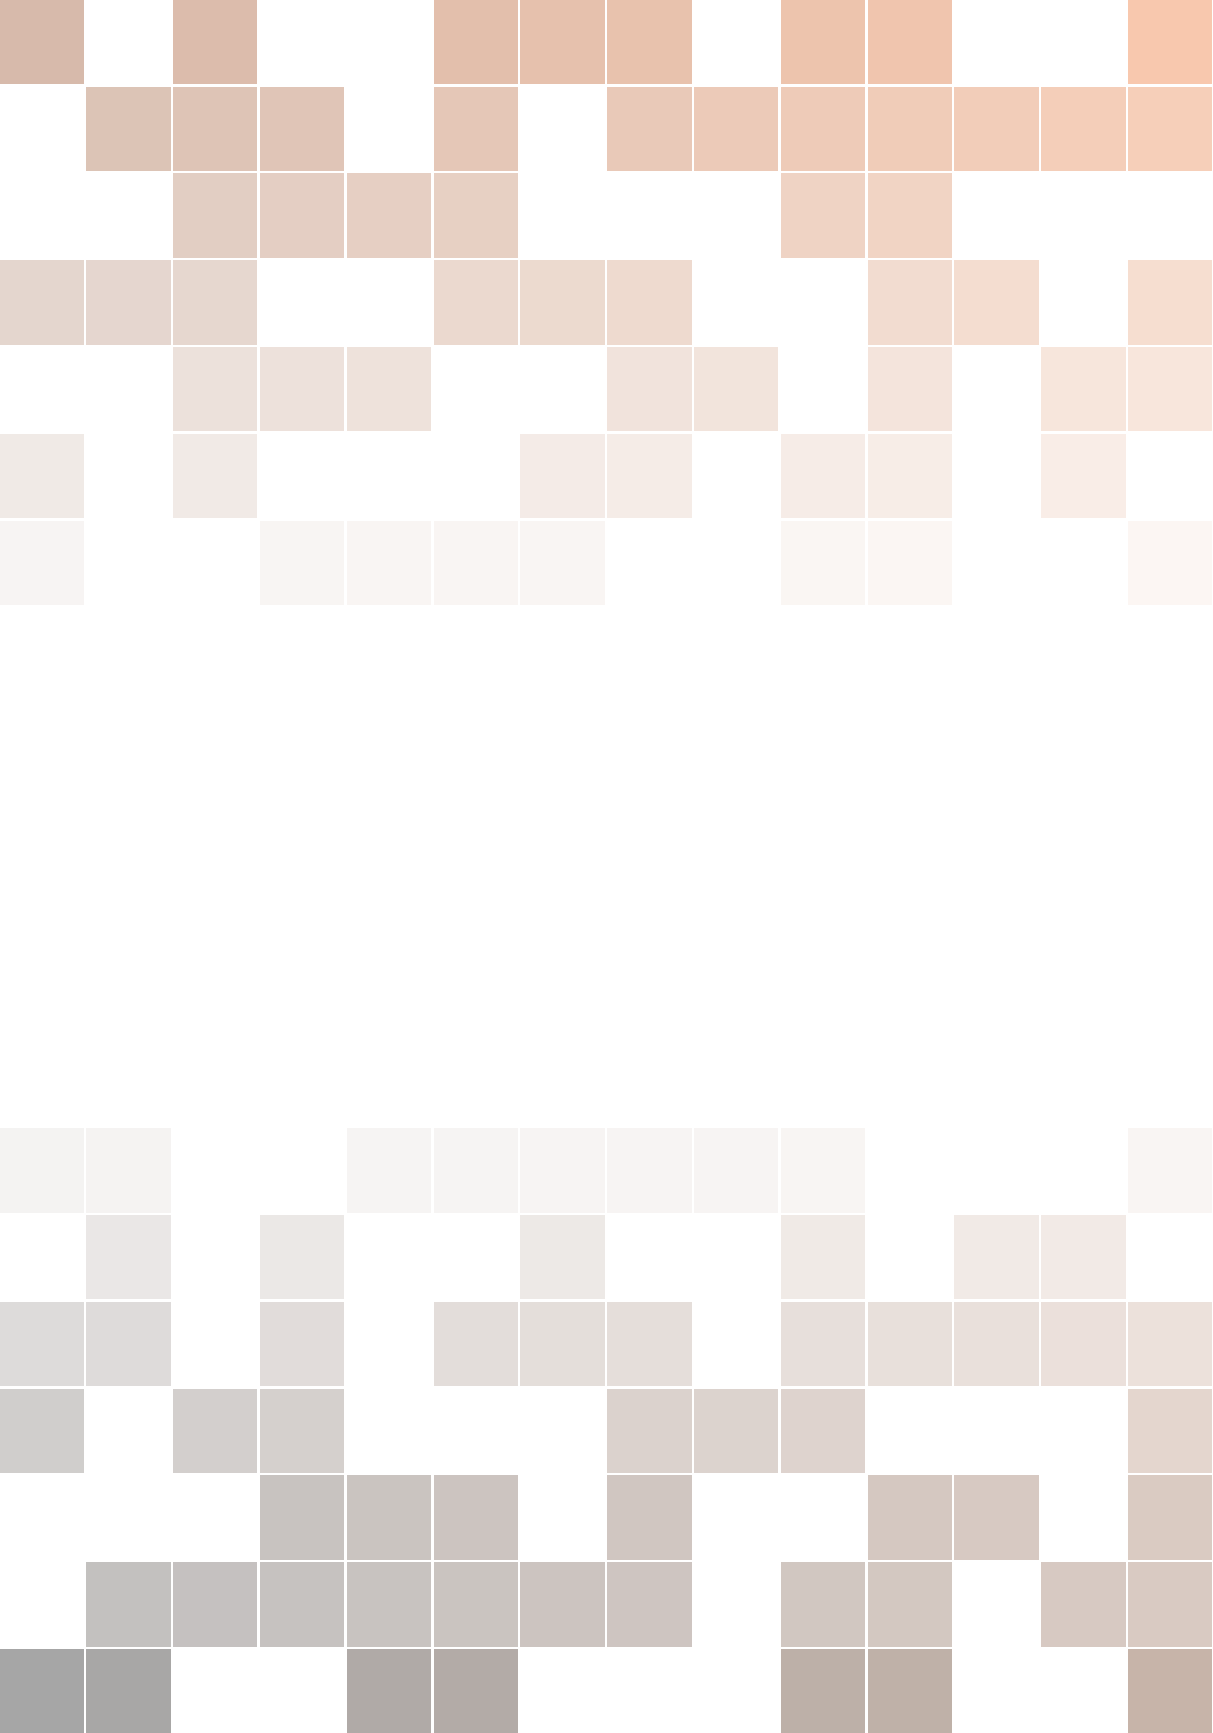
\includegraphics[scale=1]{background.pdf}}} % Image background
{\flushright
\vspace*{6cm}
\par\normalfont\fontsize{35}{35}\sffamily\selectfont

Introduzione alla \\
\vspace*{16pt}
Meccanica Statistica \\
\vspace*{32pt}
Soluzioni degli esercizi\par % Book title

\vspace*{2cm}
{\huge Marco Guagnelli}\par % Author name
}
\endgroup

%----------------------------------------------------------------------------------------
%	COPYRIGHT PAGE
%----------------------------------------------------------------------------------------

\newpage
~\vfill
\thispagestyle{empty}

\noindent Copyright \copyright\ 2014--2017 Marco Guagnelli\\ % Copyright notice

\noindent www.pv.infn.it/\textasciitilde guagnelli/ms\\ % URL

\noindent These notes have been composed using the {\em memoir} package\\

\noindent Licensed under the Creative Commons Attribution-NonCommercial 3.0 Unported License (the ``License''). You may not use this file except in compliance with the License. You may obtain a copy of the License at \url{http://creativecommons.org/licenses/by-nc/3.0}. Unless required by applicable law or agreed to in writing, software distributed under the License is distributed on an \textsc{``AS IS'' BASIS, WITHOUT WARRANTIES OR CONDITIONS OF ANY KIND}, either express or implied. See the License for the specific language governing permissions and limitations under the License.\\ % License information

\noindent \textit{Versione 1.1, Aprile 2017} % Printing/edition date
\cleardoublepage

%----------------------------------------------------------------------------------------
%	TABLE OF CONTENTS
%----------------------------------------------------------------------------------------

\pagestyle{empty} % No headers
\tableofcontents % Print the table of contents itself
\cleardoublepage % Forces the first chapter to start on an odd page so it's on the right
\pagestyle{ruled} % Print headers again

%----------------------------------------------------------------------------------------



%%%%%%%%%%%%%%%%%%%%%%%%%%%%%%%%%%%%%%%%%%%%%%%%%%%%%%%%%%%%%%%%%%%%%%%%
\chapter{Soluzioni degli esercizi del Capitolo \ref{cap:termodinamica}}
%%%%%%%%%%%%%%%%%%%%%%%%%%%%%%%%%%%%%%%%%%%%%%%%%%%%%%%%%%%%%%%%%%%%%%%%

%%%%%%%%%%%%%%%%%%%%%%%%%%%%%%%%%%%%%%%%%%%%%%%%%%%%%%%%%%%%%%%%%%%%%%%%
%
% Ricavare espressione per C_V e C_P
%
\section*{Esercizio \ref{ex:01-cvcp1}}
\addcontentsline{toc}{section}{Esercizio \ref{ex:01-cvcp1}}
%%%%%%%%%%%%%%%%%%%%%%%%%%%%%%%%%%%%%%%%%%%%%%%%%%%%%%%%%%%%%%%%%%%%%%%%

Ricordiamo il primo principio della termodinamica:
%---
\be
\label{ans1:primo}
\de U = \de Q - \de L
\ee
%---
nella quale né $\de Q$ né $\de L$ sono differenziali esatti; ma $\de U$ lo è. Per definizione abbiamo
%---
\be
C_V = \dparc{Q}{T}{V}
\ee
%---
e scrivendo $U = U(T,V)$, con una differenziazione totale otteniamo
%---
\be
\label{ans1:diffU1}
\de U = \dparc{U}{T}{V}\de T + \dparc{U}{V}{T}\de V
\ee
%---
Poiché sappiamo che per una trasformazione reversibile $\de L = P\de V$, osservando la (\ref{ans1:diffU1}) possiamo identificare subito
%---
\be
P = -\dparc{U}{V}{T}
\ee
%---
e dunque $\left.\de Q\right|_V = \left.\de U\right|_V$, cioè
%---
\be
C_V = \dparc{U}{T}{V}
\ee
%---
Per contro, esprimendo $U$ come funzione di $(T,P)$, otteniamo
%---
\be
\label{ans1:diffU1}
\de U = \dparc{U}{T}{P}\de T + \dparc{U}{P}{T}\de P
\ee
%---
Introducendo il potenziale termodinamico {\em entalpia}, $H = U + PV$, abbiamo
%---
\be
\de H = \de U + P\de V + V \de P = \de Q + V \de P
\ee
%---
È quindi chiaro che $\left.\de H\right|_P = \left.\de Q\right|_P$, da cui
%---
\be
C_P = \dparc{H}{T}{P}
\ee
%---

%%%%%%%%%%%%%%%%%%%%%%%%%%%%%%%%%%%%%%%%%%%%%%%%%%%%%%%%%%%%%%%%%%%%%%
%
% Ricavare l'equazione di stato dei gas perfetti dalle condizioni
% U dipende solo da T e non da V
% H dipende solo da T e non da P
%
\section*{Esercizio \ref{ex:01-PVNkT}}
\addcontentsline{toc}{section}{Esercizio \ref{ex:01-PVNkT}}
%%%%%%%%%%%%%%%%%%%%%%%%%%%%%%%%%%%%%%%%%%%%%%%%%%%%%%%%%%%%%%%%%%%%%%

Scriviamo i differenziali dell'energia interna $U$ e dell'entalpia $H$ in termini delle loro variabili naturali:
%---
\bea
\label{ans1:deUdeH}
\de U = T\de S - P\de V \nonumber \\
\de H = T\de S + V\de P
\eea
%---
Le due condizioni (a) e (b) menzionate nel testo dell'esercizio significano che $(\partial U/\partial V)_T = 0$ e che $(\partial H/\partial P)_T = 0$. Otteniamo quindi facilmente, dalle (\ref{ans1:deUdeH}),
%---
\be
\label{ans1:dsvt}
\dparc{S}{V}{T} = \dfrac{P}{T} \quad\quad\quad \dparc{S}{P}{T} = -\dfrac{V}{T}
\ee
%---
Possiamo liberarci dell'entropia $S$ utilizzando le relazioni di Maxwell:
%---
\be
\dparc{S}{V}{T} = \dparc{P}{T}{V} \quad\quad\quad \dparc{S}{P}{T} = -\dparc{V}{T}{P}
\ee
%---
ottenendo quindi
%---
\be
\dparc{P}{T}{V} = \dfrac{P}{T} \quad\quad\quad \dparc{V}{T}{P} = \dfrac{V}{T}
\ee
%---
Integriamo facilmente queste equazioni, ottenendo
%---
\be
P = f_1(V) T \quad\quad\quad V = f_2(P) T
\ee
%---
in cui $f_1(\cdot)$ e $f_2(\cdot)$ sono funzioni sconosciute. Ma le due equazioni devono essere contemporaneamente valide, quindi
%---
\be
\dfrac{P}{f_1(V)} = \dfrac{V}{f_2(P)} = T = \text{costante}
\ee
%---
L'unico modo perché ciò sia vero è che valga $f_1(V) = \alpha/V$ e $f_2(P) = \alpha/P$, con qualche costante $\alpha$. Possiamo dunque scrivere
%---
\be
PV = \alpha T
\ee
%---
Ci rendiamo però conto che a sinistra abbiamo una quantità estensiva; quindi anche $\alpha$ dev'essere estensiva, cioè proporzionale al numero di particelle $N$. Possiamo dunque scrivere
%---
\be
PV = N\tilde{k}T
\ee
%---
in cui la costante $\tilde{k}$ deve avere dimensioni tali che $\tilde{k}T$ sia dimensionalmente un'energia. Non ci resta che identificare $\tilde{k}$ con la costante di Boltzmann $k$. Usando l'equazione appena ottenuta e la prima delle (\ref{ans1:dsvt}) possiamo scrivere
%---
\be
\dfrac{P}{T} = \dfrac{N\tilde{k}}{V} = \dparc{S}{V}{T}
\ee
%---
Ma noi da principi primi sappiamo che l'entropia $S$ dev'essere della forma
%---
\be
S = Nk[\ln V + f_3(T)]
\ee
%---
quindi vediamo facilmente che $\tilde{k} = k$, e otteniamo $PV = NkT$.

%%%%%%%%%%%%%%%%%%%%%%%%%%%%%%%%%%%%%%%%%%%%%%%%%%%%%%%%%%%%%%%%%%%%%%
%
% Minimo dell'energia libera di Helmholtz e dell'energia libera di Gibbs
%
\section*{Esercizio \ref{ex:01-potAG}}
\addcontentsline{toc}{section}{Esercizio \ref{ex:01-potAG}}
%%%%%%%%%%%%%%%%%%%%%%%%%%%%%%%%%%%%%%%%%%%%%%%%%%%%%%%%%%%%%%%%%%%%%%

Consideriamo un sistema a volume $V$ fissato, posto a contatto con una riserva termica a temperatura costante $T$. Finché il sistema non è in equilibrio con la riserva non è possibile definire la temperatura del sistema stesso, e quindi neanche la sua energia libera di Helmholtz $A(T,V)$. Possiamo però provare a definire un'energia libera di {\em non equilibrio}:
\be
A = U - TS
\ee
in cui è inteso che $U$ è l'energia interna del sistema, definita anche fuori dall'equilibrio, e $T$ la temperatura della riserva termica. L'entropia $S$ quando il sistema non è all'equilibrio non è semplicemente una funzione di $U$ e $V$, ma dipende dai dettagli dello stato di non equilibrio. Possiamo appellarci al teorema di Clausius e scrivere
\be
\de S = \ge \de Q / T
\ee
in cui $\de Q$ è la quantità di calore trasferita dalla riserva termica al sistema. Poiché il volume è costante, avremo $\de L = 0$, e quindi $\de Q = \de U$. D'altronde la temperatura $T$ della riserva termica è costante, e quindi
\be
\de A = \de U - T \de S = \de Q - T \de S \le 0
\ee
Quindi $A$ decresce sempre, fino a che non si arriva all'equilibrio; non potendo decrescere, la condizione di equilibrio equivale a una condizione di minimo per $A$.

Allo stesso modo possiamo considerare, nel caso di un sistema a pressione costante in contatto con una riserva termica a temperatura costante $T$, l'energia libera di Gibbs, $G = U + PV - TS$. Differenziando a temperatura e pressione costanti otteniamo
\be
\de G = \de U + P\de V - T\de S
\ee
ma in questo caso abbiamo $\de U = \de Q - P\de V$. Sostituendo nella precedente otteniamo
\be
\de G = \de Q - T\de S \le 0
\ee
e possiamo svolgere le stesse considerazioni di prima circa la condizione di equilibrio e quella di minimo di $G$.

%%%%%%%%%%%%%%%%%%%%%%%%%%%%%%%%%%%%%%%%%%%%%%%%%%%%%%%%%%%%%%%%%%%%%%
%
% Esprimere C_V e C_P in termini di quantità fisiche più facili da
% misurare sperimentalmente
%
\section*{Esercizio \ref{ex:01-cvcp2}}
\addcontentsline{toc}{section}{Esercizio \ref{ex:01-cvcp2}}
%%%%%%%%%%%%%%%%%%%%%%%%%%%%%%%%%%%%%%%%%%%%%%%%%%%%%%%%%%%%%%%%%%%%%%

Scriviamo l'entropia $S$ come funzione di $T$ e $V$, ottenendo
\be
T\de S = T\dparc{S}{T}{V}\de T + T\dparc{S}{V}{T}\de V
\ee
In prima istanza notiamo che per una trasformazione a volume costante abbiamo $T\de S|_V = \de Q = C_V\de T$, e quindi
\be
T\dparc{S}{T}{V} = C_V
\ee
Per il secondo termine, consideriamo l'energia libera di Helmholtz $A(T,V)$. Dall'identità
\be
\left[\dparu{V}\dparc{A}{T}{V}\right]_T = \left[\dparu{T}\dparc{A}{V}{T}\right]_V
\ee
otteniamo la relazione di Maxwell
\be
\dparc{S}{V}{T} = \dparc{P}{T}{V}
\ee
Utilizziamo ora l'identità
\be
\dparc{P}{T}{V}\dparc{T}{V}{P}\dparc{V}{P}{T} = -1
\ee
per ottenere
\be
\dparc{S}{V}{T} = -\dfrac{(\partial V/\partial T)_P}{(\partial V/\partial P)_T} = \dfrac{\alpha}{\kappa_T}
\ee
trovando quindi
\be
\label{ans1:TdS1}
T\de S = C_V\, \de T + \dfrac{\alpha T}{\kappa_T}\de V
\ee
Allo stesso modo, considerando $S$ come funzione di $T$ e $P$, abbiamo
\be
T\de S = T\dparc{S}{T}{P}\de T + T\dparc{S}{P}{T}\de P
\ee
Per il primo termine ragioniamo come in precedenza per ottenere
\be
T\dparc{S}{T}{P} = C_P
\ee
Differenziando l'energia libera di Gibbs $G(T,P)$, otteniamo la relazione di Maxwell
\be
\dparc{S}{P}{T} = -\dparc{V}{T}{P} = -\alpha V
\ee
e quindi
\be
\label{ans1:TdS2}
T\de S = C_P\, \de T - \alpha TV\de P
\ee
Consideriamo ora una trasformazione a pressione costante: dalla (\ref{ans1:TdS1}) e dalla (\ref{ans1:TdS2}) otteniamo (ricordando che $\de P = 0$)
\be
TdS = C_V\, \de T + \dfrac{\alpha T}{\kappa_T}\de V = C_P\de T
\ee
e quindi
\be
CP - C_V = \dfrac{\alpha T}{\kappa_T}\dparc{V}{T}{P} = \dfrac{\alpha^2 TV}{\kappa_T}
\ee
Se invece consideriamo una trasformazione isoentropica, otteniamo
\bea
0 &=& C_V\, \de T|_S + \dfrac{\alpha T}{\kappa_T}\de V|_S \nonumber \\
0 &=& C_P\, \de T|_S - \alpha TV\de P|_S
\eea
Il rapporto tra queste due equazioni fornisce
\be
\dfrac{C_P}{C_V} = -V\kappa_T\dparc{P}{V}{S} = \dfrac{\kappa_T}{\kappa_S}
\ee
Abbiamo ora due equazioni in due incognite, $C_P$, e $C_V$, e risolvendo il sistema otteniamo
\bea
C_V &=& \dfrac{\alpha^2 TV \kappa_S}{\kappa_T(\kappa_T-\kappa_S)} \nonumber\\
C_P &=& \dfrac{\alpha^2 T V}{\kappa_T-\kappa_S}
\eea

%%%%%%%%%%%%%%%%%%%%%%%%%%%%%%%%%%%%%%%%%%%%%%%%%%%%%%%%%%%%%%%%%%%%%%
%
% Variazione totale di entropia per una quantità d'acqua a contatto
% con una riserva termica. Possibilità di avere un processo (ideale)
% per il quale \Delta S_{tot} = 0
%
\section*{Esercizio \ref{ex:01-pasta}}
\addcontentsline{toc}{section}{Esercizio \ref{ex:01-pasta}}
%%%%%%%%%%%%%%%%%%%%%%%%%%%%%%%%%%%%%%%%%%%%%%%%%%%%%%%%%%%%%%%%%%%%%%

Per rispondere alla domanda (a), immaginiamo, ai fini di calcolare la variazione di entropia dell'acqua, una trasformazione reversibile in cui la temperatura dell'acqua si innalza, in ciascun passo infinitesimo, di una quantità infinitesima. In ciascun passo avremo
\be
\de S_a = \dfrac{\de Q_{\text{rev}}}{T} = C\dfrac{\de T}{T}
\ee
e integrando
\be
\Delta S_a = C\int_{T_i}^{T_f} \dfrac{\de T}{T} = C\ln(T_f/T_i)
\ee
La riserva termica è invece a temperatura fissata, e quindi avremo semplicemente
\be
\Delta S_R = -\dfrac{\Delta Q}{T_f} = -C \dfrac{T_f - T_i}{T_f}
\ee
in cui $\Delta Q$ è la quantità totale di calore immessa dalla riserva nell'acqua. Sostituendo i valori numerici, $T_i = 283.15$ K e $T_f = 363.15$ K otteniamo
\be
\Delta S = \Delta S_a + \Delta S_R \simeq 0.0285 \; C
\ee

Per rispondere alla domanda (b), sviluppiamo gli stessi ragionamenti di prima, ottenendo
\be
\Delta S_a = C\left(
\ln(T_f/T_1) + \ln(T_1/T_i) = C\ln(T_f-T_i)
\right)
\ee
cioè la procedura in due passi, con una riserva termica a temperatura intermedia, non cambia la variazione di entropia dell'acqua. Per la variazione di entropia delle due riserve termiche, otteniamo invece
\bea
\Delta S_R = \Delta S_R^{(1)} + \Delta S_R^{(2)} &=& -C\left[
\dfrac{T_1-T_i}{T_1} + \dfrac{T_f-T_1}{T_f}
\right] \nonumber \\
&=& -C\left(
\dfrac{2T_f T_1 - T_f T_i - T_i^2}{T_1 T_f}
\right)
\eea
e inserendo i dati numerici per le temperature otteniamo
\be
\Delta S = \Delta S_a + \Delta S_R \simeq 0.0149 \; C
\ee

Per rispondere alla domanda (c), osserviamo che la risposta alla domanda (b) ci suggerisce di dividere l'intero processo in $N$ passi, con $N$ riserve termiche a temperature
\be
T_n = T_i + \dfrac{n}{N}(T_f-T_i) \quad\quad n = 1 \dots N
\ee
In questo modo abbiamo che la variazione di entropia di tutte le riserve termiche, alla fine del processo, sarà
\be
\Delta S_R = -C \sum_{n=1}^{N} \dfrac{T_n - T_{n-1}}{T_n}
= -C \sum_{n=1}^{N} \dfrac{(T_f-T_i)/N}{T_i + (n/N)(T_f-T_i)}
\ee
Ponendo $x \equiv (n/N)(T_f - T_i)$ e passando al limite $N\to\infty$ otteniamo
\be
\lim_{N\to\infty}\Delta S_R = - C\int_0^{T_f-T_i}\dfrac{\de x}{T_i + x} = -C\ln(T_f-T_i) = -\Delta S_a
\ee
e in questo modo abbiamo che $\Delta S = 0$.

Il risultato ci dice che abbiamo creato un processo ideale reversibile. Nella realtà dei fatti le cose non possono andare così. Prima di tutto, abbiamo assunto di poter scaldare l'acqua in maniera reversibile per calcolare $\Delta S_a$. In secondo luogo, abbiamo assunto di avere a disposizione un numero infinito di riserve termiche, con temperature che cambiano in maniera infinitesimale. Naturalmente tutto ciò rappresenta un'idealizzazione che non può in alcun modo essere realizzata in maniera pratica, e quindi per cuocere la pasta dobbiamo rassegnarci ad aumentare necessariamente l'entropia dell'Universo.

%%%%%%%%%%%%%%%%%%%%%%%%%%%%%%%%%%%%%%%%%%%%%%%%%%%%%%%%%%%%%%%%%%%%%%
%
% Calcoli termodinamici con l'eq di van der Waals
%
\section*{Esercizio \ref{ex:01-vanderWaals}}
\addcontentsline{toc}{section}{Esercizio \ref{ex:01-vanderWaals}}
%%%%%%%%%%%%%%%%%%%%%%%%%%%%%%%%%%%%%%%%%%%%%%%%%%%%%%%%%%%%%%%%%%%%%%

Per mostrare che $C_V$ è indipendente dal volume, calcoliamo $(\partial C_V/\partial V)_T$ come segue:
\bea
\dparc{C_V}{V}{T} = T\left[
\dparu{V}\dparc{S}{T}{V}
\right]_T &=& T\left[
\dparu{T}\dparc{S}{V}{T}
\right]_V \nonumber \\
&=& T\left(
\dfrac{\partial^2 P}{\partial^2 T}
\right)_V
\eea
Nel penultimo passaggio abbiamo sfruttato l'irrilevanza dell'ordine di derivazione per le derivate seconde dei potenziali termodinamici, mentre nell'ultimo abbiamo usato la relazione di Maxwell 
$(\partial S/\partial V)_T = (\partial P/\partial T)_V$. L'equazione di stato per un gas di van der Waals può essere scritta nella forma
\be
P = kTB(b,N,V) + A(a,N,V)
\ee
in cui $A$ e $B$ sono funzioni che, in prima approssimazione, non dipendono dalla temperatura. Vediamo quindi facilmente che $(\partial^2 P/\partial^2 T)_V = 0$ (ricordare che anche $N$ è fissato), da cui la risposta alla domanda (a).

Per quel che riguarda il punto (b), notiamo che l'energia interna $U$ non varia per un'espansione libera adiabatica. A differenza del gas ideale classico, però, l'energia interna non è più solo funzione della temperatura $T$. È utile considerare $U$, in tutta generalità, come una funzione della coppia $(T,V)$. Abbiamo quindi
\be
\label{ans1:deUvdW1}
\de U = \dparc{U}{T}{V}\de T + \dparc{U}{V}{T}\de V =
C_V\,\de T + \left[
T\dparc{P}{T}{V} - P
\right]\,\de V
\ee
Per ottenere il secondo termine nel membro più a destra della (\ref{ans1:deUvdW1}) abbiamo ragionato in questo modo: sappiamo che $\de U = T\de S - P\de V$ e quindi per una variazione a temperatura fissata otteniamo
\be
\dparc{U}{V}{T} = T\dparc{S}{V}{T} - P
\ee
Usando la relazione di Maxwell $(\partial S/\partial V)_T = (\partial P/\partial T)_V$ abbiamo proprio il termine cercato.

Ora, usando l'equazione di stato di van der Waals, otteniamo esplicitamente
\be
\de U = C_V\,\de T + \dfrac{aN^2}{V^2}\,\de V
\ee
Poiché $U$ non varia abbiamo $\de U = 0$ e quindi
\be
\int_{T_i}^{T_f}\de T = -\dfrac{aN^2}{C_V}\int_{V_i}^{V_f}\dfrac{\de V}{V^2}
\ee
cioè
\be
T_f - T_i = -\dfrac{aN^2}{C_V}\left(
\dfrac{1}{V_i} - \dfrac{1}{V_f}
\right)
\ee
Notiamo che se $a > 0$, come è il caso per un potenziale attrattivo a lunghe distanze, la temperatura del sistema diminuisce. Possiamo interpretare questo fatto pensando che in seguito all'espansione le particelle in media si allontaneranno le une dalle altre, incrementando l'energia potenziale tra loro; di conseguenza, poiché l'energia interna totale non cambia, l'energia cinetica, ovvero la temperatura, deve diminuire. Se $a = 0$, cioè senza potenziale attrattivo, la temperatura rimane invariata.

Consideriamo ora l'entropia come funzione della coppia $(T,V)$. Possiamo scrivere
\be
\de S = \dparc{S}{T}{V}\de T + \dparc{S}{V}{T}\de V
\ee
e usando ancora una volta, per il termine più a destra, la relazione di Maxwell citata in precedenza, otteniamo
\be
\de S = \dfrac{C_V}{T}\,\de T + \dparc{P}{T}{V}\de V
\ee
Tenendo conto dell'equazione di stato, abbiamo infine
\be
\de S = \dfrac{C_V}{T}\,\de T + \dfrac{Nk}{V - Nb}\,\de V
\ee
e integrando troviamo
\be
\Delta S = \int_i^f = C_V\ln\left(\dfrac{T_f}{T_i}\right) + 
Nk\ln\left(\dfrac{V_f-Nb}{V_i-Nb} \right)
\ee
Sostituendo nella precedente il risultato per la temperatura finale $T_f$ otteniamo finalmente
\be
\Delta S = C_V\ln\left(1 - \dfrac{aN^2}{C_V T_i}\left(\dfrac{1}{V_i}-\dfrac{1}{V_f}\right)\right)
+ Nk\ln\left(\dfrac{V_f-Nb}{V_i-Nb} \right)
\ee

%%%%%%%%%%%%%%%%%%%%%%%%%%%%%%%%%%%%%%%%%%%%%%%%%%%%%%%%%%%%%%%%%%%%%%

\vskip 0.75cm
\begin{flushright}
{\em Ultimo aggiornamento del capitolo: 22.04.2017}
\end{flushright}
%%%%%%%%%%%%%%%%%%%%%%%%%%%%%%%%%%%%%%%%%%%%%%%%%%%%%%%%%%%%%%%%%%%%%%%%
\chapter{Soluzioni degli esercizi del Capitolo \ref{cap:basi}}
%%%%%%%%%%%%%%%%%%%%%%%%%%%%%%%%%%%%%%%%%%%%%%%%%%%%%%%%%%%%%%%%%%%%%%%%

%%%%%%%%%%%%%%%%%%%%%%%%%%%%%%%%%%%%%%%%%%%%%%%%%%%%%%%%%%%%%%%%%%%%%%%%
\section*{Esercizio \ref{ex:02-relaSOmega}}
\addcontentsline{toc}{section}{Esercizio \ref{ex:02-relaSOmega}}
%%%%%%%%%%%%%%%%%%%%%%%%%%%%%%%%%%%%%%%%%%%%%%%%%%%%%%%%%%%%%%%%%%%%%%%%

Data la natura additiva di $S$ e moltiplicativa di $\Omega$ la funzione $f$ deve necessariamente soddisfare la relazione
\be
\label{ans2:o1o2}
f(\Omega_1\Omega_2) = f(\Omega_1) + f(\Omega_2)
\ee
Differenziando la precedente sia rispetto a $\Omega_1$ sia rispetto a $\Omega_2$ otteniamo le due equazioni
\be
\Omega_2 f'(\Omega_1\Omega_2) = f'(\Omega_1) \quad\quad
\Omega_1 f'(\Omega_1\Omega_2) = f'(\Omega_2)
\ee
Dividendo l'una per l'altra otteniamo
\be
\Omega_1 f'(\Omega_1) = \Omega_2 f'(\Omega_2)
\ee
Ma il termine a sinistra dell'equazione è indipendente da $\Omega_2$, mentre il termine a destra è indipendente da $\Omega_1$. Poiché sono uguali, entrambi i termini devono necessariamente essere una costante $k$ indipendente sia da $\Omega_1$ sia da $\Omega_2$. Abbiamo dunque
\be
f'(\Omega) = \dfrac{k}{\Omega}
\ee
e cioè
\be
f(\Omega) = k\ln(\Omega) + c
\ee
in cui $c$ è una costante di integrazione. Inserendo l'ultima equazione nella (\ref{ans2:o1o2}) vediamo subito che $c=0$.

%%%%%%%%%%%%%%%%%%%%%%%%%%%%%%%%%%%%%%%%%%%%%%%%%%%%%%%%%%%%%%%%%%%%%%%%
\section*{Esercizio \ref{ex:02-sfere}}
\addcontentsline{toc}{section}{Esercizio \ref{ex:02-sfere}}
%%%%%%%%%%%%%%%%%%%%%%%%%%%%%%%%%%%%%%%%%%%%%%%%%%%%%%%%%%%%%%%%%%%%%%%%

Costruiamo il nostro sistema aggiungendo una particella alla volta. Il primo atomo, trascurando effetti di bordo, avrà a disposizione un volume $V$. Per il secondo atomo occorre considerare il volume già occupato dal primo; avrà quindi a disposizione un volume pari a $(V-\alpha v_0)$, con $\alpha$ da determinare. Osservando la figura \ref{fig:02-sol-raggio2} si evince subito che il volume escluso è quello di una sfera di raggio $2r$, e cioè $8v_0$. 
%%%%%%%%%%%%%%%%%%%%%%%%%%%%%%%%%%%%%%%%%%%%%%%%%%%%%%%%%%%%%%%%%%%%%%
\begin{figure}[!ht]
\centering
  \begin{tikzpicture}[scale=0.5]
  \draw[thick,blue,fill=blue!20] (0,0) circle (2);
  \draw[thick,blue,fill=blue!20] (4,0) circle (2);
  \draw[thick,red,dotted] (0,0) circle (4);
  \draw[thick,dashed] (0,0)--(4,0);
  \draw (1,-0.3) node{$r$};
  \draw (3,-0.3) node{$r$};
\end{tikzpicture}


  \caption{Effetti di volume escluso.}
  \label{fig:02-sol-raggio2}
\end{figure}
%%%%%%%%%%%%%%%%%%%%%%%%%%%%%%%%%%%%%%%%%%%%%%%%%%%%%%%%%%%%%%%%%%%%%%
Dunque $\alpha = 8$. Per la dipendenza del numero dei microstati dal volume otteniamo dunque subito
\bea
\Omega &\propto& V(V-8v_0)(V-16v_0)\cdots(V-8kv_0)\cdots(V-8(N-1)v_0) \nonumber\\
	   &=& \prod_{k=0}^{N-1}(V-8kv_0)
\eea
Abbiamo quindi, con $C$ indipendente dal volume $V$, 
\bea
\ln\Omega &=& \sum_{k=0}^{N-1}\ln(V-8kv_0) + C = \sum_{k=0}^{N-1}\ln[V(1-8kv_0/V)] + C \nonumber\\
&\simeq& N\ln V -\frac{8v_0}{V}\sum_{k=0}^{N} k + C
\eea
in cui nell'ultimo passaggio abbiamo approssimato $N-1\simeq N$ e abbiamo espanso il logaritmo, $\ln(1+x) = x + \cdots$.
L'ultima sommatoria nella precedente vale $N(N+1)/2$, che approssimiamo con $N^2/2$. Otteniamo quindi, per l'entropia,
\be
S = kN\left\{ \ln V - \frac{4Nv_0}{V} \right\} + kC
\ee
Utilizziamo ora la formula
\be
\frac{P}{T} = \dparc{S}{V}{N,E}
\ee
per ottenere
\be
P = \frac{NkT}{V}\left\{ 1 + \frac{4Nv_0}{V} \right\}
\ee
Troviamo quindi un volume efficace pari a
\be
V_{\textrm{eff}} = \frac{V}{1+4Nv_0/V} \simeq V\left\{ 1 - \frac{4Nv_0}{V} \right\} = V-4Nv_0
\ee
che è esattamente il risultato che ci eravamo proposti di dimostrare.

%%%%%%%%%%%%%%%%%%%%%%%%%%%%%%%%%%%%%%%%%%%%%%%%%%%%%%%%%%%%%%%%%%%%%%%%
\section*{Esercizio \ref{ex:02-Saddit}}
\addcontentsline{toc}{section}{Esercizio \ref{ex:02-Saddit}}
%%%%%%%%%%%%%%%%%%%%%%%%%%%%%%%%%%%%%%%%%%%%%%%%%%%%%%%%%%%%%%%%%%%%%%%%

Se $S$ è estensiva sappiamo che dev'essere direttamente proporzionale a $N$, cioè
\be
S(E,N,V) = Nf(E,V)
\ee
A questo punto però la rimanente funzione $f(E,V)$ dev'essere in realtà funzione di $(E/N,V/N) \equiv (\eps, v)$:
\be
S(E,N,V) = Nf(\eps, v)
\ee
Abbiamo dunque:
\bea
N\dparc{S}{N}{E,V} &=& N\left[
f(\eps,v) + N\dparc{f}{\eps}{v}\dpar{\eps}{N} + N\dparc{f}{v}{\eps}\dpar{v}{N}
\right] \nonumber \\
&=& N\left[
f(\eps,v) - \dparc{f}{\eps}{v}\dfrac{E}{N} - \dparc{f}{v}{\eps}\dfrac{V}{N}
\right] \nonumber \\
E\dparc{S}{E}{N,V} &=& NE\dparc{f}{\eps}{v}\dpar{\eps}{N} = E\dparc{f}{\eps}{v} \nonumber \\
V\dparc{S}{V}{E,V} &=& NV\dparc{f}{v}{\eps}\dpar{v}{N} = V\dparc{f}{v}{\eps}
\eea
Sommando le tre espressioni otteniamo il risultato cercato.

%%%%%%%%%%%%%%%%%%%%%%%%%%%%%%%%%%%%%%%%%%%%%%%%%%%%%%%%%%%%%%%%%%%%%%%%

\vskip 0.75cm
\begin{flushright}
{\em Ultimo aggiornamento del capitolo: 22.04.2017}
\end{flushright}

%%%%%%%%%%%%%%%%%%%%%%%%%%%%%%%%%%%%%%%%%%%%%%%%%%%%%%%%%%%%%%%%%%%%%%%%
\chapter{Soluzioni degli esercizi del Capitolo \ref{cap:elementi}}
%%%%%%%%%%%%%%%%%%%%%%%%%%%%%%%%%%%%%%%%%%%%%%%%%%%%%%%%%%%%%%%%%%%%%%%%

%%%%%%%%%%%%%%%%%%%%%%%%%%%%%%%%%%%%%%%%%%%%%%%%%%%%%%%%%%%%%%%%%%%%%%%%
\section*{Esercizio \ref{ex:03-gicur}}
\addcontentsline{toc}{section}{Esercizio \ref{ex:03-gicur}}
%%%%%%%%%%%%%%%%%%%%%%%%%%%%%%%%%%%%%%%%%%%%%%%%%%%%%%%%%%%%%%%%%%%%%%%%

Per una particella relativistica di massa $m$ la relazione di dispersione energia--impulso è:
%---
\be
\varepsilon^2 = p^2c^2 + m^2c^4
\ee
%---
in cui $c$ è la velocità della luce. Il caso ultrarelativistico corrisponde a trascurare la massa rispetto al momento. Otteniamo dunque
%---
\be
\varepsilon = pc
\ee
%---
in cui $p$ è il modulo del momento. L'hamiltoniana totale per un gas ultrarelativistico sarà dunque
%---
\be
\Ham = \sum_{i=1}^N p_i c
\ee
%---
Passiamo al calcolo del numero di microstati con energia minore o uguale a $E$. Abbiamo
%---
\be
\Sigma(E) = \frac{1}{N!}\frac{1}{h^{3N}}\int\limits_{\sum_i p_i \le P}\de^{3N} q \, \de^{3N} p
\ee
%---
in cui abbiamo posto $P\equiv E/c$. L'integrazione sulle coordinate fornisce semplicemente un fattore $V^N$ perché $\Ham$ non dipende dalle coordinate. Inoltre riscriviamo $\de^3 p = 4\pi p^2\de p$ ottenendo
%---
\be
\Sigma(E) = \frac{1}{N!}\frac{(4\pi V)^N}{h^{3N}}\int\limits_{\sum_i p_i \le P}\prod_{i=1}^N p_i^2\,\de p_i
\ee
%---
Consideriamo l'integrale nell'espressione precedente nel caso semplificato $N=2$; possiamo scrivere
%---
\be
I_2(P) = \int p_1^2\,\de p_1\int p_2^2\,\de p_2 \,\theta(P - p_1 - p_2)
\ee
%---
in cui $\theta$ è la funzione a gradino. Riscriviamo quindi
%---
\be
I_2(P) = \int_0^P p_1^2\,\de p_1\int_0^{P-p_1} p_2^2\, \de p_2 = \frac{1}{3}\int_0^P p_1^2(P-p_1)^3\de p_1
\ee
%---
Risolviamo l'integrale più generale
%---
\be
J_A(P) = \int_0^P x^2(P-x)^A\de x
\ee
%---
che ci farà comodo in seguito. Poniamo $y = (P-x)$ e otteniamo subito
%---
\be
J_A(P) = \int_0^P(y^{A+2} - 2Py^{A+1} + P^2y^A)\de y
\ee
%---
e un facile calcolo ci fornisce il risultato:
%---
\be
\label{eq:JA}
J_A(P) = \frac{2A!}{(A+3)!}P^{A+3}
\ee
%---
Abbiamo dunque
%---
\be
I_2(P) = \frac{1}{3}J_3(P) = \frac{2^2}{6!}P^6
\ee
%---
Il motivo per cui abbiamo scritto il risultato in questa maniera sarà chiaro tra poco. Consideriamo ora $I_3(P)$; si vede facilmente, utilizzando il risultato \ref{eq:JA} che abbiamo
%---
\be 
I_3(P) = \int_0^P p_1^2 I_2(P-p_1)\de p_1 = \frac{2^3 6!}{6! 9!}P^9 = \frac{2^3}{9!}P^9
\ee
%---
Procedendo iterativamente otteniamo
%---
\be
I_N(P) = \int_0^P p_1^2 \,I_{N-1}(P-p_1)\de p_1 = \frac{2^N}{(3N)!}P^{3N}
\ee
%---
e dunque l'espressione per il volume dello spazio delle fasi
%---
\be
\Sigma(E) = \frac{1}{N!}\frac{(8\pi V)^N E^{3N}}{(3N)!(hc)^{3N}}
\ee
%---
Abbiamo già visto che possiamo usare direttamente $\Sigma(E)$ per calcolare l'entropia: otteniamo dunque, utilizzando la formula di Stirling
%---
\be
\label{eq:sgum}
S(E,N,V) = Nk\left[
\ln\left(\frac{8\pi VE^3}{27(hc)^3 N^4}\right) + 4
\right]
\ee 
%---
Notiamo che se avessimo omesso il fattore correttivo di Gibbs nel logaritmo sarebbe apparsa la quantità
$VE^3/N^3$ invece che $VE^3/N^4$; la seconda espressione rende l'entropia una grandezza estensiva, la prima no.

Per una trasformazione adiabatica abbiamo $S = \mathrm{costante}$, e dunque $VE^3 = 
\mathrm{costante}$. Ricordando che
%---
\be
P = -\dparc{E}{V}{S}
\ee
%---
otteniamo subito
%---
\be
P = \frac{E}{3V}
\ee
%---
Ricaviamo inoltre anche la legge per una trasformazione adiabatica:
%---
\be
PV^{4/3} = \mathrm{costante}
\ee
%---
da cui si legge subito
%---
\be
\frac{C_P}{C_V}\equiv\gamma = \frac{4}{3}
\ee
%---

%%%%%%%%%%%%%%%%%%%%%%%%%%%%%%%%%%%%%%%%%%%%%%%%%%%%%%%%%%%%%%%%%%%%%%%%
\section*{Esercizio \ref{ex:03-oscfermi}}
\addcontentsline{toc}{section}{Esercizio \ref{ex:03-oscfermi}}
%%%%%%%%%%%%%%%%%%%%%%%%%%%%%%%%%%%%%%%%%%%%%%%%%%%%%%%%%%%%%%%%%%%%%%%%

Sia $N_{+}$ il numero di particelle nello stato di energia $\varepsilon$ e $N_{-}$ il numero di particelle nello stato di energia $-\varepsilon$. Abbiamo chiaramente che
\be
\label{eq:es0}
N = N_{+} + N_{-}
\ee
e inoltre possiamo scrivere
\be
\label{eq:es1}
E = \varepsilon(N_{+} - N_{-}) = \varepsilon (2N_{+} - N)
\ee
Calcoliamo l'entropia con la formula di Boltzmann,
\be
S = k\ln \Gamma(E)
\ee
in cui $\Gamma(E)$ è il numero di microstati compatibili con il macrostato di energia $E$. 

Da notare che in questo caso $\Gamma(E)$ non va diviso per $h^N$ perché lo ``spazio delle fasi'' del sistema è già discreto e $\Gamma(E)$ è un numero puro, adimensionale.

Per calcolare $\Gamma(E)$ dobbiamo contare in quanti modi possiamo distribuire le $N$ particelle tra i due livelli in modo che valga la (\ref{eq:es1}), e la risposta è
%---
\be
\Gamma(E) = \frac{N!}{N_{+}!N_{-}!} = \frac{N!}{N_{+}!(N-N_{+})!}
\ee
%---
Utilizzando la formula di Stirling otteniamo subito
%---
\be
S = k\left[N\ln N - N_{+}\ln N_{+} - (N-N_{+})\ln(N-N_{+})\right]
\ee
%---
Per ottenere l'inverso della temperatura d'equilibrio dobbiamo derivare $S$ rispetto a $E$, cioè in definitiva rispetto alla variabile $(2\varepsilon N_{+})$:
%---
\be
\frac{1}{T} = \frac{1}{2\varepsilon}\dpar{S}{N_{+}} = \frac{k}{2\varepsilon}
\left[ \ln\frac{N-N_{+}}{N_{+}} \right]
\ee
%---
dalla quale otteniamo subito la prima risposta:
%---
\be
\label{eq:es2}
N_{+} = \frac{N}{1+e^{2\varepsilon/kT}}
\ee
%---
e la (\ref{eq:es0}) ci permette subito di scrivere
%---
\be
N_{-} = \frac{Ne^{2\varepsilon/kT}}{1+e^{2\varepsilon/kT}}
\ee
%---
Nel limite $T\to 0$ il denominatore delle espressioni precedenti è dominato dall'esponenziale, e otteniamo quindi subito:
%---
\be
\lim_{T\to 0}N_{+} = 0\qquad\qquad \lim_{T\to 0}N_{-} = N
\ee
%---
e cioè solo il livello a energia inferiore è popolato. Invece per $T\to\infty$ otteniamo
%---
\be
\lim_{T\to\infty}N_{\pm} = \frac{N}{2}
\ee
%---
e cioè entrambi i livelli sono ugualmente popolati. Per l'energia ciò implica che a $T=0$ il sistema raggiunge l'energia minima, ossia $E = -\varepsilon N$, mentre il valore massimo (in una situazione d'equilibrio termodinamico), $E = 0$, viene raggiunto solo a temperatura infinita. Ne segue che sistemi a energia positiva sono necessariamente fuori dall'equilibrio.

Se l'energia vale $E$, possiamo scrivere $N_{+} = (E+N\varepsilon)/2\varepsilon$, e possiamo quindi esprimere l'entropia $S$ in funzione di $E$:
%---
\be
\label{eq:SE}
\frac{S(E)}{Nk} = -\frac{N\varepsilon + E}{2N\varepsilon}\ln\left(\frac{N\varepsilon + E}{2N\varepsilon}\right)
-\frac{N\varepsilon - E}{2N\varepsilon}\ln\left(\frac{N\varepsilon - E}{2N\varepsilon}\right)
\ee
%---
Possiamo semplificare l'espressione ponendo $\bar\varepsilon \equiv E/N\varepsilon$ e $s(\bar\varepsilon) \equiv S(E)/Nk$, ottenendo
\be
\label{eq:sol03-s-vs-e}
s(\bar\varepsilon) = \ln 2 - \dfrac{1}{2}\left[
(1+\bar\varepsilon)\ln(1+\bar\varepsilon) + (1-\bar\varepsilon)\ln(1-\bar\varepsilon)
\right]
\ee
%%%%%%%%%%%%%%%%%%%%%%%%%%%%%%%%%%%%%%%%%%%%%%%%%%%%%%%%%%%%%%%%%%%%%%%%%
\begin{figure}[h]
  \centering
  \begin{tikzpicture}[domain=-0.999:0.999,scale=5]
  \draw[->] (-1,0) -- (1.1,0)   node[anchor=north] {$\bar\varepsilon$};
  \draw[->] (-1,0) -- (-1,0.85) node[anchor=east]  {$s(\bar\varepsilon)$};
  
  \draw[dotted,color=red] (-1,0.69314718056) -- (0,0.69314718056);
  \draw[dotted] (0,0) -- (0,0.69314718056);
  \draw (-1,-0.05) node{$-1$};
  \draw (0.001,-0.05) node{$0$};
  \draw (1,-0.05) node{$1$};
  \draw (-1.08,0.69314718056) node{$\ln 2$};
  
  \draw[thick,color=blue,samples=100,smooth] plot[id=03-s-vs-e] function{log(2)-0.5*((1+x)*log(1+x)+(1-x)*log(1-x))};
\end{tikzpicture}

  \caption{La densità di entropia, $s(\bar\varepsilon) \equiv S(E)/Nk$, in funzione di $\bar\varepsilon \equiv \varepsilon E/N$.} 
  \label{fig:03-sol-s-vs-e}
\end{figure}
%%%%%%%%%%%%%%%%%%%%%%%%%%%%%%%%%%%%%%%%%%%%%%%%%%%%%%%%%%%%%%%%%%%%%%%%%%
\noindent
La (\ref{eq:sol03-s-vs-e}) è graficata in figura \ref{fig:03-sol-s-vs-e}, e poiché la derivata di $S(E)$ rispetto a $E$ dà l'inverso della temperatura termodinamica assoluta, vediamo che stati con $E > 0$ corrispondono a $T < 0$. Visto che l'energia totale del sistema è limitata dall'alto non c'è nessun motivo teorico per non ammettere temperature negative (se non fosse limitata, uno stato a temperatura negativa potrebbe avere peso di Boltzmann infinito). Ma una temperatura negativa, poiché corrisponde a stati con energia maggiore degli stati a temperatura positiva, è sempre {\em maggiore} di qualsiasi temperatura positiva. In altre parole, se mettiamo a contatto un sistema a temperatura negativa (quindi in uno stato metastabile) con una riserva termica a temperatura positiva, il calore fluirà dal sistema a temperatura negativa a quello a temperatura positiva, e l'equilibrio termico totale si raggiungerà comunque per valori positivi della temperatura $T$.

%%%%%%%%%%%%%%%%%%%%%%%%%%%%%%%%%%%%%%%%%%%%%%%%%%%%%%%%%%%%%%%%%%%%%%%%
\section*{Esercizio \ref{ex:03-quasioscfermi}}
\addcontentsline{toc}{section}{Esercizio \ref{ex:03-quasioscfermi}}
%%%%%%%%%%%%%%%%%%%%%%%%%%%%%%%%%%%%%%%%%%%%%%%%%%%%%%%%%%%%%%%%%%%%%%%%

Definiamo $x = n_1/N$ e scriviamo $E = x\varepsilon N$. In questo modo è possibile ricavare il numero di occupazione in funzione della temperatura tramite la relazione 
\be
\label{eq:sol03oneoverT}
\dparc{S}{E}{N,V} = \dfrac{1}{\varepsilon N}\dparc{S}{x}{N,V} = \dfrac{1}{T}
\ee
Per calcolare l'entropia del sistema $S(E)$ dobbiamo determinare il numero di microstati $\Omega$ a $(E,N)$ fissati. Tale numero è dato dal numero di modi i cui possiamo scegliere $n_1$ particelle tra $N$ totali, senza che conti l'ordine di scelta; dunque dalla distribuzione di probabilità binomiale:
\be
\Omega(E,N) = \binom{N}{n_1}g^{n_1} = \dfrac{N!}{n_1!n_0!}g^{n_1}
\ee 
e nella precedente $g^{n_1}$ conta il numero di modi di distribuire $n_1$ particelle su $g$ stati degeneri.
L'entropia sarà data dalla formula di Boltzmann $S(E,N) = k\ln\Omega(E,N)$:
\be
  \begin{split}
    S(E,N) &=      k\ln\Omega(E,N) = k [ \ln(N!g^{n_1}) - \ln n_1! - \ln((N-n_1)!) ] \\
	       &\simeq k [ N\ln N + n_1\ln g - n_1\ln n_1 - (N-n_1)\ln(N-n_1)]
%	       &= kN[\ln N + x\ln g - x\ln n + (1-\frac{n}{N})\ln(N-n)] \\
%   	       &= kN[\ln N +\frac{n}{N}\ln g - \frac{n}{N}\ln n - \ln(N(1-\frac{n}{N})) + \frac{n}{N}\ln\left(N\left[1-\frac{n}{N}\right]\right)] \\
%			&= kN[\ln N +x\ln g - x\ln n -\ln N - \ln(1-x) + x\ln N +x\ln(1-x)] \\   	       
%	       &= -kN[(1-x)\ln(1-x)+x\ln x -x\ln g]
  \end{split}
\ee
nella quale abbiamo ovviamente usato la formula di Stirling. Mettendo in evidenza un fattore $N$ e scrivendo $x$ al posto di $n_1/N$, dopo pochi passaggi otteniamo
\be
S(E,N) = kN [ x\ln g - x\ln x - (1-x)\ln(1-x) ]
\ee
Abbiamo dunque, usando la (\ref{eq:sol03oneoverT}),
\be
	\beta = \dfrac{1}{kT} = \frac{1}{\varepsilon}[\ln g - \ln x - \ln(1-x) ]
\ee
da cui possiamo ricavare $x$, e quindi $n_1$, in funzione di $\beta$, e quindi di $T$:
\be
	\ln\left(\dfrac{g(1-x)}{x}\right) = \beta\varepsilon \implies x = \frac{n_1}{N} = \dfrac{g\,e^{-\beta\varepsilon}}{1 + e^{-\beta\varepsilon}}
\ee
rispondendo così al primo quesito posto dal problema:
\begin{align*}
  n_1 &=  N\dfrac{g\,e^{-\beta\varepsilon}}{1 + e^{-\beta\varepsilon}}\\
  n_0 &= 1 - n_1
\end{align*}

Per quel che riguarda il secondo quesito, abbiamo $E=0.75\,N\epsilon \implies x = 3/4$. Con $g=2$ troviamo che la temperatura del sistema
\be
  \beta\epsilon = \ln\left( \dfrac{g(1-x)}{x} \right) = \ln(2/3) \simeq -0.405 < 0
\ee
	Ciò non deve meravigliare: questo risultato implica semplicemtne che sistema è in uno stato metastabile in cui $3/4$ delle particelle si trova al livello eccitato di energia e il valore negativo della temperatura indica che il calore, nel caso di contatto con una riserva termica all'equilibrio, e quindi a temperatura sanamente positiva, fluirà \emph{dal} sistema \emph{alla} riserva di calore. In questo caso particolare si ha che ciò succederà fino a che 
\be
	\dfrac{g(1-x)}{x} < 1 \implies x > \dfrac{2}{3}, \quad \text{cioè} \quad n_1 > \dfrac{2}{3}N.
\ee 
	 Calcolando l'entropia e assumendo un flusso di energia finito tra il sistema e la riserva (S $\rightarrow$ R), abbiamo che
\be
	\Delta S = \Delta S_R - \Delta S_S = \left(\dfrac{\partial S_R}{\partial E} -\dfrac{\partial S_S}{\partial E}\right)\Delta E = \left(\dfrac{1}{T_R} -\dfrac{1 }{T_S}\right)\Delta E
\ee
	Dato che $\Delta S \ge 0$ per $\Delta E >0$ dobbiammo avere $1/T_R - 1/T_S > 0$. Vediamo dunque che le temeperature negative rientrano perfettamente in questo schema.

%%%%%%%%%%%%%%%%%%%%%%%%%%%%%%%%%%%%%%%%%%%%%%%%%%%%%%%%%%%%%%%%%%%%%%%%
\section*{Esercizio \ref{ex:03-spin1}}
\addcontentsline{toc}{section}{Esercizio \ref{ex:03-spin1}}
%%%%%%%%%%%%%%%%%%%%%%%%%%%%%%%%%%%%%%%%%%%%%%%%%%%%%%%%%%%%%%%%%%%%%%%%

Anticipando i tempi, troviamo subito la soluzione col formalismo dell'ensemble canonico. Sia $Q_1$ la funzione di partizione di singola particella. La probabilità che la particella sia nello stato $\sigma = -1$ è data da
\be
P(-1) = e^{-h/kT}/Q_1
\ee
e analogamente abbiamo
\be
P(1) = e^{h/kT}/Q_1
\ee
Poiché $N_{-1} = NP(-1)$ e $N_{1} = NP(1)$, otteniamo subito
\be
\label{exeq:ratiocan}
\dfrac{N_{-1}}{N_{1}} = e^{-2h/kT}
\ee

Le particelle sono distinguibili e non--interagenti, quindi per la funzione di partizione totale del sistema, $Q_N$, possiamo scrivere
\be
Q_N = Q_1^N
\ee
Il calcolo di $Q_1$ è immediato:
\be
Q_1 = e^{-h/kT} + 1 + e^{h/kT}
\ee
Per l'energia libera di Helmholtz troviamo:
\be
A = -kT\ln Q_N = -NkT \ln Q_1 = -NkT \ln\left(e^{-h/kT} + 1 + e^{h/kT}\right).
\ee

Il conto col formalismo microcanonico è molto più complicato. Per semplicità di notazione, poniamo $X \equiv N_{0}$, $Y \equiv N_{1}$, $Z \equiv N_{-1}$ e $\calE \equiv E/h$.

Possiamo scrivere i vincoli su $N$ e su $E$, entrambi fissati:
\bea
\label{exeq:vinc1}
N &=& X + Y + Z \nonumber \\
\calE &=& Z - Y
\eea
Immaginiamo ora di fissare $X$: ci restano $N-X$ particelle che possono essere distribuite sui due livelli rimanenti. Il numero di modi in cui possiamo fare ciò è chiaramente
\be
\Omega'(X,Y,Z) = \dfrac{(N-X)!}{Y!Z!} = \dfrac{(N-X)!}{Y!(N-X-Y)!}
\ee
Per ottenere il numero di microstati totali non ci resta che contare tutti i modi in cui possiamo scegliere $X$ particelle tra $N$, moltiplicare per $\Omega'$ e sommare su tutti i possibili valori di $X$:
\be
\Omega(X,Y,Z) = \sum_{X=?}^{?} \dfrac{N!}{X!(N-X)!}\dfrac{(N-X)!}{Y!(N-X-Y)!} =
\sum_{X=?}^{?} \dfrac{N!}{X!Y!Z!}
\ee

Il primo problema è quello di trovare i limiti della sommatoria su $X$. I vincoli (\ref{exeq:vinc1}) ci permettono di scrivere:
\be
X = N - \calE - 2Y
\ee
dalla quale ricaviamo che il limite inferiore della somma su $X$ è uguale a $0$ se $N-\calE$ è pari, mentre è uguale a $1$ in caso contrario. L'ultima equazione ci mostra anche che il limite superiore della somma su $X$ corrisponde al valore minimo di $Y$: osserviamo però, notando che $Y = Z-\calE$, che $\text{min}\{Y\} = 0$ se $\calE \ge 0$, mentre $\text{min}\{Y\} = -\calE$ se $\calE < 0$. Si vede subito che il limite superiore nella somma su $X$ è pari a $N-|\calE|$. Abbiamo quindi
\be
\Omega(X,Y,Z) = \sum_{X=(0 || 1}^{N-|\calE|} \dfrac{N!}{X!Y!Z!} \equiv \sum_{X=(0 || 1}^{N-|\calE|}
\Phi(X,\calE,N)
\ee

Come al solito, non sappiamo fare questa somma. Un argomento di tipo {\em punto di sella} mostra però che nel limite termodinamico ($N\to\infty$) possiamo sostituire alla somma il termine che massimizza la funzione $\Phi$. Prima di ottenere il valore di $X_0$ che massimizza $\Phi$, e quindi $\ln\Phi$, osserviamo che a $X$ fissato abbiamo
\bea
\label{exeq:YZ}
Y = \dfrac{N-\calE-X}{2} \nonumber \\
Z = \dfrac{N+\calE-X}{2}
\eea

Usando la formula di Stirling abbiamo
\be
\ln\Phi = N\ln N - X\ln X - Y\ln Y - Z\ln Z
\ee
e quindi
\be
\label{exeq:max}
\dparc{\ln\Phi}{X}{X=X_0} = -(\ln(X_0)+1) - \dfrac{1}{2}(\ln(Y_0)+1) - \dfrac{1}{2}(\ln(Z_0)+1) = 0
\ee
in cui abbiamo usato la notazione $Y_0 \equiv Y(X_0)$, $Z_0 \equiv Z(X_0)$ e il fatto che
\be
\dpar{Y}{X} = \dpar{Z}{X} = -\dfrac{1}{2}
\ee
La soluzione dell'equazione (\ref{exeq:max}) è
\be
X_0^2 = Y_0 Z_0
\ee
e ponendo $x_0 \equiv X_0/N$, $y_0 \equiv Y_0/N$, $z_0 \equiv Z_0/N$ e infine $\eps \equiv \calE/N$, otteniamo
\be
x_0^2 = y_0 z_0
\ee
e infine, usando le (\ref{exeq:YZ}), troviamo
\be
x_0 = \dfrac{1}{3}\left(\sqrt{4-3\eps^2}-1\right)
\ee
Per l'entropia del sistema otteniamo
\be
S = k\ln\Phi(X_0,\calE,N) = k(N\ln N - X_0\ln X_0 - Y_0\ln Y_0 - Z_0\ln Z_0)
\ee
e definendo $s \equiv S/Nk$ abbiamo
\be
s = \ln N - x_0\ln(Nx_0) - y_0\ln(Ny_0) - y_0\ln(Nz_0)
\ee
Ma ricordando che $x_0 + y_0 + z_0 = 1$ otteniamo facilmente
\be
s = - x_0\ln x_0 - y_0\ln y_0 - y_0\ln z_0
\ee
Troviamo la temperatura d'equilibrio del sistema con la formula
\be
\beta = \dfrac{1}{kT} = \dfrac{1}{k}\dparc{S}{E}{N} = \dfrac{1}{h}\dpar{s}{\eps}
\ee
e quindi
\be
\dfrac{h}{kT} = -(\ln y_0 + 1)\dpar{y_0}{\eps}-(\ln z_0 + 1)\dpar{z_0}{\eps}
\ee
e usando ancora le (\ref{exeq:YZ}) otteniamo
\be
\dfrac{2h}{kT} = -\ln(z_0/y_0)
\ee
Abbiamo finalmente
\be
\dfrac{N_{-1}}{N_{1}} = \dfrac{z_0}{y_0} = e^{-2h/kT}
\ee
da confrontare con la (\ref{exeq:ratiocan}).

Definiamo ora $r \equiv e^{-h/kT}$. Abbiamo $z_0/y_0 = r^2$ e $x_0^2 = y_0z_0$, da cui ricaviamo facilmente $x_0^2/r^2 = y_0z_0/r^2 = y_0^2$, e cioè
\bea
y_0 &=& x_0/r \nonumber \\
z_0 &=& x_0 r \nonumber \\
x_0 &=& (r^{-1} + 1 + r)^{-1}
\eea
in cui l'ultima è stata ricavata ricordando che $x_0 + y_0 + z_0 = 1$. Con un po' di manipolazioni riusciamo a ottenere
\bea
S &=& -Nk \left[
\ln x_0 + x_0(r-r^{-1})\ln r
\right] \nonumber \\
U &=& Nh\eps = Nh(z_0-y_0) = Nhx_0(r-r^{-1}) \nonumber \\
T &=& -\dfrac{h}{k\ln r}
\eea
e quindi
\be
A = U - TS = -NkT \ln\left(e^{-h/kT} + 1 + e^{h/kT}\right)
\ee
e cioè lo stesso risultato del canonico ma usando una quantità di calcoli ben più pesante.

%%%%%%%%%%%%%%%%%%%%%%%%%%%%%%%%%%%%%%%%%%%%%%%%%%%%%%%%%%%%%%%%%%%%%%

\vskip 0.75cm
\begin{flushright}
{\em Ultimo aggiornamento del Capitolo: 22.04.2017}
\end{flushright}

%%%%%%%%%%%%%%%%%%%%%%%%%%%%%%%%%%%%%%%%%%%%%%%%%%%%%%%%%%%%%%%%%%%%%%%%
\chapter{Soluzione degli esercizi del Capitolo \ref{cap:canonico}}
%%%%%%%%%%%%%%%%%%%%%%%%%%%%%%%%%%%%%%%%%%%%%%%%%%%%%%%%%%%%%%%%%%%%%%%%

%%%%%%%%%%%%%%%%%%%%%%%%%%%%%%%%%%%%%%%%%%%%%%%%%%%%%%%%%%%%%%%%%%%%%%%%
\section*{Esercizio \ref{ex:04-guc}}
\addcontentsline{toc}{section}{Esercizio \ref{ex:04-guc}}
%%%%%%%%%%%%%%%%%%%%%%%%%%%%%%%%%%%%%%%%%%%%%%%%%%%%%%%%%%%%%%%%%%%%%%%%
Scriviamo, come al solito per sistemi non interagenti,
\be
Q_N(V,T) = \frac{1}{N!}[Q_1(V,T)]^N
\ee
con $Q_1$ funzione di partizione di singola particella. Abbiamo
\be
Q_1(V,T) = \frac{1}{h^3}\int \de^3 q\int \de^3 p \,e^{-\beta pc}
\ee
e quindi possiamo calcolare immediatamente
\be
Q_1(V,T) = \frac{8\pi V}{(\beta hc)^3}
\ee
L'energia libera di Helmholtz è
\be
A(V,T) = -kT\ln Q_N(V,T) = -kTN
\left\{
\ln\left( \frac{8\pi V(kT)^3}{N(hc)^3} \right)
\right\}
\ee
Otteniamo subito
\be
\label{eq:pguc}
P = -\dparc{A}{V}{N,T} = \frac{NkT}{V}
\ee
ovvero l'equazione di stato (identica a quella del gas non relativistico). Per l'energia abbiamo invece
\be
\label{eq:uguc}
U = -\dpar{\ln Q_N}{\beta} = 3NkT
\ee
La relazione tra pressione, volume ed energia è quindi $PV = U/3$. Passando all'entropia, abbiamo
\be
S = \frac{U-A}{T}
\ee
e con pochi passaggi otteniamo subito
\be
S = Nk
\left\{
\ln\left( \frac{8\pi V(kT)^3}{N(hc)^3} \right) + 4
\right\}
\ee
Se vogliamo confrontarci con il risultato microcanonico, cioè con l'eq. (\ref{eq:sgum}), dobbiamo inserire nella precedente l'energia interna; dalla (\ref{eq:uguc}) otteniamo subito
\be
S(U,N,V) = Nk\left\{\ln\left(\frac{8\pi VU^3}{27(hc)^3 N^4}\right) + 4\right\}
\ee
Se consideriamo $S = \mathrm{costante}$, allora abbiamo l'implicazione $VU^3 = \mathrm{costante}$ (per $N = \mathrm{costante}$), e otteniamo subito, usando la (\ref{eq:pguc}), il rapporto $C_P/C_V$:
\be
PV^{4/3} = \mathrm{costante} \quad
\gamma \equiv C_P/C_V = 4/3
\ee
Per la densità degli stati abbiamo
\be
g(E) = \frac{1}{2\pi i}\oint e^{\beta E}Q(\beta)\de\beta
\ee
in cui abbiamo già previsto di chiudere l'integrale di linea sul piano complesso nella direzione $\beta\to -\infty$. Si trova facilmente
\be
g(E) = \frac{1}{N!}
\left\{
\frac{8\pi V}{(hc)^3}
\right\}^N \frac{1}{2\pi i}\oint \frac{e^{\beta E}}{\beta^{3N}} \simeq
\frac{1}{N!}
\left\{
\frac{8\pi VE^3}{(hc)^3}
\right\}^N
\ee
in cui nell'ultimo passaggio abbiamo usato $3N-1 \simeq 3N$ (limite termodinamico).

%%%%%%%%%%%%%%%%%%%%%%%%%%%%%%%%%%%%%%%%%%%%%%%%%%%%%%%%%%%%%%%%%%%%%%%%
\section*{Esercizio \ref{ex:04-oscfermi}}
\addcontentsline{toc}{section}{Esercizio \ref{ex:04-oscfermi}}
%%%%%%%%%%%%%%%%%%%%%%%%%%%%%%%%%%%%%%%%%%%%%%%%%%%%%%%%%%%%%%%%%%%%%%%%
La funzione di partizione di singola particella è:
\be
Q_1 = e^{-\beta\varepsilon} + e^{\beta\varepsilon} = 2 \cosh(\beta\varepsilon)
\ee
Troviamo subito il numero di occupazione per i due livelli:
\bea
N_{-} &=& N \dfrac{e^{\beta\varepsilon}}{e^{-\beta\varepsilon} + e^{\beta\varepsilon}}
= \dfrac{N}{1 + e^{-2\beta\varepsilon}} \nonumber \\
N_{+} &=& N \dfrac{e^{-\beta\varepsilon}}{e^{-\beta\varepsilon} + e^{\beta\varepsilon}}
= \dfrac{N}{1 + e^{2\beta\varepsilon}}
\eea

%%%%%%%%%%%%%%%%%%%%%%%%%%%%%%%%%%%%%%%%%%%%%%%%%%%%%%%%%%%%%%%%%%%%%%%%
\section*{Esercizio \ref{ex:04-eqchim}}
\addcontentsline{toc}{section}{Esercizio \ref{ex:04-eqchim}}
%%%%%%%%%%%%%%%%%%%%%%%%%%%%%%%%%%%%%%%%%%%%%%%%%%%%%%%%%%%%%%%%%%%%%%%%

All'equilibrio termodinamico i potenziali chimici devono essere uguali da entrambi i lati della reazione, quindi
\be
	\label{eq:sol04-mueq}
	\mu_a + \mu_b = \mu_{ab}
\ee
	Sappiamo che 
\be
	\mu_x = \dparc{A_x}{N_x}{T,V}= -kT\dparc{\ln Q(N_x)}{N_x}{T,V}
\ee
	La funzione di partizione per un gas ideale classico è data da
\be
	Q(N_x) = \dfrac{1}{N_x!}\left[Q_x\right]^{N_x}
\ee
	quindi, usando la formula di Stirling, 
\be
	\mu_x = -kT\dparu{N_x}\left[ N_x\ln Q_x - N_x\ln N_x + N_x \right] = -kT[\ln Q_x - \ln N_x]
\ee
	Sostituendo nella (\ref{eq:sol04-mueq}) e ricordando che $N_x = n_x V$ si ottiene facilmente
\be 
	\ln{\dfrac{Q_a Q_b}{Q_{ab}}}= \ln \dfrac{N_a N_b}{N_{ab}} \quad\rightarrow\quad 
	\dfrac{n_{ab}}{n_a n_b} = V\dfrac{Q_{ab}}{Q_{a}Q_{b}}
\ee

%%%%%%%%%%%%%%%%%%%%%%%%%%%%%%%%%%%%%%%%%%%%%%%%%%%%%%%%%%%%%%%%%%%%%%%%
\section*{Esercizio \ref{ex:04-esps}}
\addcontentsline{toc}{section}{Esercizio \ref{ex:04-esps}}
%%%%%%%%%%%%%%%%%%%%%%%%%%%%%%%%%%%%%%%%%%%%%%%%%%%%%%%%%%%%%%%%%%%%%%%%
Abbiamo visto  che l'entropia di un gas ideale classico vale
\be
\frac{S}{Nk} = \ln\left(\frac{V}{N\lambda^3}\right) + \frac{5}{2}
\ee
in cui $\lambda$ è la lunghezza d'onda termica (o di de Broglie). Ai fini dell'esercizio ci basta ricordare che
\be
\lambda^3 = cT^{-3/2}
\ee
con $c$ indipendente dalla temperatura $T$,  per cui ricordando che $Q_1 = V/\lambda^3$ possiamo scrivere
\be
\ln\left(\frac{Q_1}{N}\right) + T\dparc{\ln Q_1}{T}{P} =
\ln\left(\frac{V}{N\lambda^3}\right) + 3/2 + \frac{T}{V}\dparc{V}{T}{P}
\ee
Per un gas ideale abbiamo la relazione $V = NkT/P$, quindi
\be
\frac{T}{V}\dparc{V}{T}{P} = \frac{NkT}{PV} = 1
\ee
da cui discende ciò che dovevamo dimostrare.
%%%%%%%%%%%%%%%%%%%%%%%%%%%%%%%%%%%%%%%%%%%%%%%%%%%%%%%%%%%%%%%%%%%%%%%%
\chapter{Soluzioni degli esercizi del Capitolo \ref{cap:grancanonico}}
%%%%%%%%%%%%%%%%%%%%%%%%%%%%%%%%%%%%%%%%%%%%%%%%%%%%%%%%%%%%%%%%%%%%%%%%

%%%%%%%%%%%%%%%%%%%%%%%%%%%%%%%%%%%%%%%%%%%%%%%%%%%%%%%%%%%%%%%%%%%%%%%%
\section*{Esercizio \ref{ex:05-eqcgc}}
\addcontentsline{toc}{section}{Esercizio \ref{ex:05-eqcgc}}
%%%%%%%%%%%%%%%%%%%%%%%%%%%%%%%%%%%%%%%%%%%%%%%%%%%%%%%%%%%%%%%%%%%%%%%%

La funzione di partizione canonica per $N$ particelle non interagenti è
\be
Q_N(T,V) = \left[ Q_1(T,V) \right]^N
\ee
Dalla precedente otteniamo subito
\be
\label{eq:sol05-AC}
\begin{split}
U_C &= -\dparc{\ln Q_N}{\beta}{N,V} = NkT^2 \dfrac{Q_1'}{Q_1} \\
A_C &= -kT\ln Q_N = -NkT\ln Q_1 \\
S_C &= \dfrac{U_C - A_C}{T} = Nk\left(
T\dfrac{Q_1'}{Q_1} + \ln Q_1
\right)
\end{split}
\ee
nelle quali $Q_1' = (\partial Q_1/\partial T)_{V}$.

Per la funzione di partizione grancanonica abbiamo invece
\be
\calQ(z,T,V) = \sum_{N=0}^\infty [ z Q_1 ]^N = \dfrac{1}{1 - zQ_1}
\ee
Per poter confrontare i risultati del canonico con quelli del grancanonico, dobbiamo aggiustare la fugacità $z$ in modo tale che valga la relazione
\be
N = \aspetta{N}_G = z\dparc{\ln\calQ}{z}{T,V} = \dfrac{zQ_1}{1 - zQ_1}
\ee
e ciò implica facilmente
\be
zQ_1 = \dfrac{N}{N+1} \quad\quad \mu = -kT\ln\left( \dfrac{(N+1)Q_1}{N} \right)
\ee
Questo ci permette di scrivere il granpotenziale $q$ come una funzione di $(N,T)$:
\be
q = kT\ln\calQ = kT\ln(N+1)
\ee
e per le prime due grandezze termodinamiche di interesse otteniamo
\be
\label{eq:sol05-AG}
\begin{split}
U_G &= -\dparc{q}{\beta}{z,V} = NkT^2 \dfrac{Q_1'}{Q_1} \\
A_G &= \mu N - q = kT [ N\ln N - (N+1)\ln(N+1) - N\ln Q_1
\end{split}
\ee
Abbiamo chiaramente che $U_G = U_C$ e quindi, utilizzando la seconda delle (\ref{eq:sol05-AC}) e la seconda delle (\ref{eq:sol05-AG}), otteniamo facilmente
\be
\frac{S_G-S_C}{Nk} = -\frac{A_G-A_C}{NkT} \simeq \frac{\ln N}{N}
\ee

%%%%%%%%%%%%%%%%%%%%%%%%%%%%%%%%%%%%%%%%%%%%%%%%%%%%%%%%%%%%%%%%%%%%%%%%
\section*{Esercizio \ref{ex:05-sas}}
\addcontentsline{toc}{section}{Esercizio \ref{ex:05-sas}}
%%%%%%%%%%%%%%%%%%%%%%%%%%%%%%%%%%%%%%%%%%%%%%%%%%%%%%%%%%%%%%%%%%%%%%%%

La funzione di partizione grancanonica del gas ideale classico racchiuso nel contenitore è
\be
\calQ(z,T,V) = \sum_{N=0}^{\infty} \dfrac{1}{N!}[z Q_1]^N = e^{zQ_1}
\ee
in cui $Q_1(T,V) = V/\lambda^3 = V(2\pi mkT/h^2)^{3/2}$ è la funzione di partizione canonica di singola particella. Applicando la formula
\be
q = \ln\calQ(z,T,V) = \dfrac{PV}{NkT}
\ee
otteniamo subito la pressione
\be
P = z\left(\dfrac{2\pi m}{h^2}\right)^{3/2}(kT)^{5/2}
\ee
e da quest'ultima possiamo ricavare la fugacità del gas:
\be
z_g = P(kT)^{-5/2}\left(\dfrac{h^2}{2\pi m}\right)^{3/2}
\ee
Dal punto di vista dell'ensemble grancanonico, sia il gas sia ciascun centro di assorbimento sulle pareti del contenitore sono in contatto con una riserva, termica e di particelle, caratterizzata da temperatura $T$ e fugacità $z$, che saranno quindi le stesse per il gas e per i centri di assorbimento. Scriviamo la funzione di granpartizione di un singolo sito di assorbimento:
\be
\calQ_s = \sum_{N=0}{1}(z_s e^{\beta\varepsilon})^N = 1 + ze^{\beta\varepsilon}
\ee
Il numero medio di molecole assorbite dalle pareti, considerando $N_0$ siti di assorbimento, sarà dunque
\be
\aspetta{N_a} = N_0 z_s\dparc{\calQ_s}{z_s}{T} = \dfrac{N_0}{1+z_s^{-1}e^{-\beta\varepsilon}}
\ee
Per trovare $\aspetta{N_a}$ in funzione della pressione $P$ del gas basterà uguagliare $z_s = z_g$, trovando
\be
\aspetta{N_a} = \dfrac{N_0}{1 + (2\pi m/h^2)^{3/2} P^{-1}(kT)^{5/2}e^{-\beta\varepsilon}}
\ee
Risulta chiaro che a temperatura $T$ fissata, per pressione molto alta $\aspetta{N_a}$ tenderà a saturare al valore $N_0$, mentre per pressione molto bassa $\aspetta{N_a} \simeq 0$.


%%%%%%%%%%%%%%%%%%%%%%%%%%%%%%%%%%%%%%%%%%%%%%%%%%%%%%%%%%%%%%%%%%%%%%

\vskip 0.75cm
\begin{flushright}
{\em Ultimo aggiornamento del Capitolo: 22.04.2017}
\end{flushright}

\end{document}
